\documentclass{article}

\usepackage[final]{neurips}


\usepackage[utf8]{inputenc} % allow utf-8 input
\usepackage[T1]{fontenc}    % use 8-bit T1 fonts
\usepackage{hyperref}       % hyperlinks
\usepackage{url}            % simple URL typesetting
\usepackage{booktabs}       % professional-quality tables
\usepackage{amsfonts}   
\usepackage{amsmath}
\usepackage{mathtools}% blackboard math symbols
\usepackage{nicefrac}       % compact symbols for 1/2, etc.
\usepackage{microtype}      % microtypography
\usepackage{graphicx}
\usepackage{xepersian}
\settextfont{XB Yas.ttf}
\title{صفحه 35}

\author{%

  نرم افزار ریاضی\\

  \texttt{@gmail.com} \\
}


\begin{document}
\baselineskip=0.7cm

\begin{minipage}{0.1\textwidth}% adapt widths of minipages to your needs

\includegraphics[width=1.2cm]{Amirkabir.jpg}
\end{minipage}%
\hfill%
\begin{minipage}{0.9\textwidth}\raggedleft
دانشگاه صنعتی امیرکبیر\\
مباحث ویژه در بهینه سازی\\
\end{minipage}

\makepertitle
\begin{flushleft}
$min  q(x)=(x-1 - 1)^2+(x_2 - 2.5)^2$\\
  
\begin{tabular}{ r | c  l }
$q_1$\hspace{5mm}$-x_1+2x_2<=2$   &   s.t.  \\
$q_2$\hspace{5mm}$x_1+2x_2<=6 $&\\
$q_3$\hspace{5mm} $x_1-2x_2<=2$ &\\
$q_4$\hspace{5mm}  $-x_1<=0$  &\\
$q_5$\hspace{5mm}   $-x_2<=0$  &\\

\end{tabular}


\end{flushleft}
حل:
\begin{flushleft}
$H=
\begin{bmatrix}
2 & 0\\
0 & 2
\end{bmatrix}
\hspace{10mm}
C=
\begin{bmatrix}
-2\\
-5
\end{bmatrix}$
\end{flushleft}
\begin{flushleft}
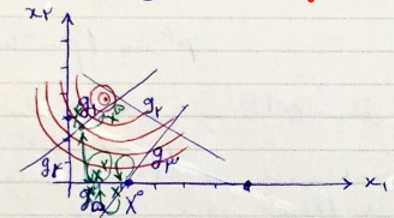
\includegraphics[width=10cm]{Diagram.png}\\
\end{flushleft}


\centering
\begin{tabular}{l l l l l l}
k & $x^k$     & $w^k$               & $p^k$     & $\alpha^k$ & $\mu^j , j\in w^k$                                \\
0 & (2,0)     & \{3,5\}             & (0,0)     & \_         & $\mu_3=-2$,$\mu_5=-1$ \\
1 & (2,0)     & \{5\}               & (1,0)     & 1          & \_                                                \\
2 & (1,0)     & \{5\}               & (0,0)     & \_         &$\mu_5=-5$                          \\
3 & (1,0)     & $\phi$              & (0,2.5)   & 0.6        & \_                                                \\
4 & (1,1.5)   & \{1\}               & (0.4,0.2) & 1          & \_                                                \\
5 & (1.4,1.7) & \{1\}               &           &            & \_                                               
\end{tabular}\\
\begin{flushright}


\pagebreak
با نقطه شدنی
$\dot{X}=(2,0)$
شروع می کنیم ، داریم
$A(\dot{X})={3,5}$
و مجموعه کاری 
$\dot{W}$
را به صورت {3,5}
در نطر می گیریم
تکرار اول : در این حالت زیر مساله 
(**)
به فرم زیر است.\\
\end{flushright}

$min  q=p_1^2+p_2^2-2p_1-5*p_2$\\
$s.t. p_1-2p_2=0$\\
$-p_2=0$


\end{document}
